% Options for packages loaded elsewhere
\PassOptionsToPackage{unicode}{hyperref}
\PassOptionsToPackage{hyphens}{url}
\PassOptionsToPackage{dvipsnames,svgnames,x11names}{xcolor}
%
\documentclass[
  letterpaper,
  DIV=11,
  numbers=noendperiod]{scrartcl}

\usepackage{amsmath,amssymb}
\usepackage{iftex}
\ifPDFTeX
  \usepackage[T1]{fontenc}
  \usepackage[utf8]{inputenc}
  \usepackage{textcomp} % provide euro and other symbols
\else % if luatex or xetex
  \usepackage{unicode-math}
  \defaultfontfeatures{Scale=MatchLowercase}
  \defaultfontfeatures[\rmfamily]{Ligatures=TeX,Scale=1}
\fi
\usepackage{lmodern}
\ifPDFTeX\else  
    % xetex/luatex font selection
\fi
% Use upquote if available, for straight quotes in verbatim environments
\IfFileExists{upquote.sty}{\usepackage{upquote}}{}
\IfFileExists{microtype.sty}{% use microtype if available
  \usepackage[]{microtype}
  \UseMicrotypeSet[protrusion]{basicmath} % disable protrusion for tt fonts
}{}
\makeatletter
\@ifundefined{KOMAClassName}{% if non-KOMA class
  \IfFileExists{parskip.sty}{%
    \usepackage{parskip}
  }{% else
    \setlength{\parindent}{0pt}
    \setlength{\parskip}{6pt plus 2pt minus 1pt}}
}{% if KOMA class
  \KOMAoptions{parskip=half}}
\makeatother
\usepackage{xcolor}
\setlength{\emergencystretch}{3em} % prevent overfull lines
\setcounter{secnumdepth}{-\maxdimen} % remove section numbering
% Make \paragraph and \subparagraph free-standing
\makeatletter
\ifx\paragraph\undefined\else
  \let\oldparagraph\paragraph
  \renewcommand{\paragraph}{
    \@ifstar
      \xxxParagraphStar
      \xxxParagraphNoStar
  }
  \newcommand{\xxxParagraphStar}[1]{\oldparagraph*{#1}\mbox{}}
  \newcommand{\xxxParagraphNoStar}[1]{\oldparagraph{#1}\mbox{}}
\fi
\ifx\subparagraph\undefined\else
  \let\oldsubparagraph\subparagraph
  \renewcommand{\subparagraph}{
    \@ifstar
      \xxxSubParagraphStar
      \xxxSubParagraphNoStar
  }
  \newcommand{\xxxSubParagraphStar}[1]{\oldsubparagraph*{#1}\mbox{}}
  \newcommand{\xxxSubParagraphNoStar}[1]{\oldsubparagraph{#1}\mbox{}}
\fi
\makeatother

\usepackage{color}
\usepackage{fancyvrb}
\newcommand{\VerbBar}{|}
\newcommand{\VERB}{\Verb[commandchars=\\\{\}]}
\DefineVerbatimEnvironment{Highlighting}{Verbatim}{commandchars=\\\{\}}
% Add ',fontsize=\small' for more characters per line
\usepackage{framed}
\definecolor{shadecolor}{RGB}{241,243,245}
\newenvironment{Shaded}{\begin{snugshade}}{\end{snugshade}}
\newcommand{\AlertTok}[1]{\textcolor[rgb]{0.68,0.00,0.00}{#1}}
\newcommand{\AnnotationTok}[1]{\textcolor[rgb]{0.37,0.37,0.37}{#1}}
\newcommand{\AttributeTok}[1]{\textcolor[rgb]{0.40,0.45,0.13}{#1}}
\newcommand{\BaseNTok}[1]{\textcolor[rgb]{0.68,0.00,0.00}{#1}}
\newcommand{\BuiltInTok}[1]{\textcolor[rgb]{0.00,0.23,0.31}{#1}}
\newcommand{\CharTok}[1]{\textcolor[rgb]{0.13,0.47,0.30}{#1}}
\newcommand{\CommentTok}[1]{\textcolor[rgb]{0.37,0.37,0.37}{#1}}
\newcommand{\CommentVarTok}[1]{\textcolor[rgb]{0.37,0.37,0.37}{\textit{#1}}}
\newcommand{\ConstantTok}[1]{\textcolor[rgb]{0.56,0.35,0.01}{#1}}
\newcommand{\ControlFlowTok}[1]{\textcolor[rgb]{0.00,0.23,0.31}{\textbf{#1}}}
\newcommand{\DataTypeTok}[1]{\textcolor[rgb]{0.68,0.00,0.00}{#1}}
\newcommand{\DecValTok}[1]{\textcolor[rgb]{0.68,0.00,0.00}{#1}}
\newcommand{\DocumentationTok}[1]{\textcolor[rgb]{0.37,0.37,0.37}{\textit{#1}}}
\newcommand{\ErrorTok}[1]{\textcolor[rgb]{0.68,0.00,0.00}{#1}}
\newcommand{\ExtensionTok}[1]{\textcolor[rgb]{0.00,0.23,0.31}{#1}}
\newcommand{\FloatTok}[1]{\textcolor[rgb]{0.68,0.00,0.00}{#1}}
\newcommand{\FunctionTok}[1]{\textcolor[rgb]{0.28,0.35,0.67}{#1}}
\newcommand{\ImportTok}[1]{\textcolor[rgb]{0.00,0.46,0.62}{#1}}
\newcommand{\InformationTok}[1]{\textcolor[rgb]{0.37,0.37,0.37}{#1}}
\newcommand{\KeywordTok}[1]{\textcolor[rgb]{0.00,0.23,0.31}{\textbf{#1}}}
\newcommand{\NormalTok}[1]{\textcolor[rgb]{0.00,0.23,0.31}{#1}}
\newcommand{\OperatorTok}[1]{\textcolor[rgb]{0.37,0.37,0.37}{#1}}
\newcommand{\OtherTok}[1]{\textcolor[rgb]{0.00,0.23,0.31}{#1}}
\newcommand{\PreprocessorTok}[1]{\textcolor[rgb]{0.68,0.00,0.00}{#1}}
\newcommand{\RegionMarkerTok}[1]{\textcolor[rgb]{0.00,0.23,0.31}{#1}}
\newcommand{\SpecialCharTok}[1]{\textcolor[rgb]{0.37,0.37,0.37}{#1}}
\newcommand{\SpecialStringTok}[1]{\textcolor[rgb]{0.13,0.47,0.30}{#1}}
\newcommand{\StringTok}[1]{\textcolor[rgb]{0.13,0.47,0.30}{#1}}
\newcommand{\VariableTok}[1]{\textcolor[rgb]{0.07,0.07,0.07}{#1}}
\newcommand{\VerbatimStringTok}[1]{\textcolor[rgb]{0.13,0.47,0.30}{#1}}
\newcommand{\WarningTok}[1]{\textcolor[rgb]{0.37,0.37,0.37}{\textit{#1}}}

\providecommand{\tightlist}{%
  \setlength{\itemsep}{0pt}\setlength{\parskip}{0pt}}\usepackage{longtable,booktabs,array}
\usepackage{calc} % for calculating minipage widths
% Correct order of tables after \paragraph or \subparagraph
\usepackage{etoolbox}
\makeatletter
\patchcmd\longtable{\par}{\if@noskipsec\mbox{}\fi\par}{}{}
\makeatother
% Allow footnotes in longtable head/foot
\IfFileExists{footnotehyper.sty}{\usepackage{footnotehyper}}{\usepackage{footnote}}
\makesavenoteenv{longtable}
\usepackage{graphicx}
\makeatletter
\def\maxwidth{\ifdim\Gin@nat@width>\linewidth\linewidth\else\Gin@nat@width\fi}
\def\maxheight{\ifdim\Gin@nat@height>\textheight\textheight\else\Gin@nat@height\fi}
\makeatother
% Scale images if necessary, so that they will not overflow the page
% margins by default, and it is still possible to overwrite the defaults
% using explicit options in \includegraphics[width, height, ...]{}
\setkeys{Gin}{width=\maxwidth,height=\maxheight,keepaspectratio}
% Set default figure placement to htbp
\makeatletter
\def\fps@figure{htbp}
\makeatother

\KOMAoption{captions}{tableheading}
\makeatletter
\@ifpackageloaded{caption}{}{\usepackage{caption}}
\AtBeginDocument{%
\ifdefined\contentsname
  \renewcommand*\contentsname{Table of contents}
\else
  \newcommand\contentsname{Table of contents}
\fi
\ifdefined\listfigurename
  \renewcommand*\listfigurename{List of Figures}
\else
  \newcommand\listfigurename{List of Figures}
\fi
\ifdefined\listtablename
  \renewcommand*\listtablename{List of Tables}
\else
  \newcommand\listtablename{List of Tables}
\fi
\ifdefined\figurename
  \renewcommand*\figurename{Figure}
\else
  \newcommand\figurename{Figure}
\fi
\ifdefined\tablename
  \renewcommand*\tablename{Table}
\else
  \newcommand\tablename{Table}
\fi
}
\@ifpackageloaded{float}{}{\usepackage{float}}
\floatstyle{ruled}
\@ifundefined{c@chapter}{\newfloat{codelisting}{h}{lop}}{\newfloat{codelisting}{h}{lop}[chapter]}
\floatname{codelisting}{Listing}
\newcommand*\listoflistings{\listof{codelisting}{List of Listings}}
\makeatother
\makeatletter
\makeatother
\makeatletter
\@ifpackageloaded{caption}{}{\usepackage{caption}}
\@ifpackageloaded{subcaption}{}{\usepackage{subcaption}}
\makeatother

\ifLuaTeX
  \usepackage{selnolig}  % disable illegal ligatures
\fi
\usepackage{bookmark}

\IfFileExists{xurl.sty}{\usepackage{xurl}}{} % add URL line breaks if available
\urlstyle{same} % disable monospaced font for URLs
\hypersetup{
  pdftitle={Problem-Set-1 for POLI 271},
  colorlinks=true,
  linkcolor={blue},
  filecolor={Maroon},
  citecolor={Blue},
  urlcolor={Blue},
  pdfcreator={LaTeX via pandoc}}


\title{Problem-Set-1 for POLI 271}
\author{}
\date{}

\begin{document}
\maketitle


\section{1. Univariate displays \& sampling
distributions}\label{univariate-displays-sampling-distributions}

\subsection{\texorpdfstring{\emph{Problem
a}}{Problem a}}\label{problem-a}

\begin{Shaded}
\begin{Highlighting}[]
\NormalTok{s\_values }\OtherTok{=} \FunctionTok{c}\NormalTok{(}\DecValTok{10}\NormalTok{, }\DecValTok{100}\NormalTok{, }\DecValTok{1000}\NormalTok{)}
\NormalTok{n\_values }\OtherTok{=} \FunctionTok{c}\NormalTok{(}\DecValTok{10}\NormalTok{, }\DecValTok{100}\NormalTok{, }\DecValTok{1000}\NormalTok{)}

\FunctionTok{par}\NormalTok{(}\AttributeTok{mfrow =} \FunctionTok{c}\NormalTok{(}\DecValTok{3}\NormalTok{, }\DecValTok{3}\NormalTok{))}
\ControlFlowTok{for}\NormalTok{ (s }\ControlFlowTok{in}\NormalTok{ s\_values) \{}
  \ControlFlowTok{for}\NormalTok{ (n }\ControlFlowTok{in}\NormalTok{ n\_values) \{}
\NormalTok{    sample\_means }\OtherTok{=} \FunctionTok{replicate}\NormalTok{(s, }\FunctionTok{mean}\NormalTok{(}\FunctionTok{sample}\NormalTok{(}\DecValTok{1}\SpecialCharTok{:}\DecValTok{20}\NormalTok{, n, }\AttributeTok{replace =} \ConstantTok{TRUE}\NormalTok{)))}

    \FunctionTok{hist}\NormalTok{(sample\_means,}
         \AttributeTok{breaks =} \DecValTok{20}\NormalTok{,}
         \AttributeTok{col =} \StringTok{"grey"}\NormalTok{,}
         \AttributeTok{border =} \StringTok{"black"}\NormalTok{,}
         \AttributeTok{main =} \FunctionTok{paste}\NormalTok{(}\StringTok{"s ="}\NormalTok{, s, }\StringTok{", n ="}\NormalTok{, n),}
         \AttributeTok{xlab =} \StringTok{""}\NormalTok{,}
         \AttributeTok{xlim =} \FunctionTok{c}\NormalTok{(}\DecValTok{1}\NormalTok{, }\DecValTok{20}\NormalTok{))}
    
    \FunctionTok{abline}\NormalTok{(}\AttributeTok{v =} \FunctionTok{mean}\NormalTok{(sample\_means), }\AttributeTok{col =} \StringTok{"red"}\NormalTok{, }\AttributeTok{lwd =} \FloatTok{0.5}\NormalTok{)}
\NormalTok{  \}}
\NormalTok{\}}
\end{Highlighting}
\end{Shaded}

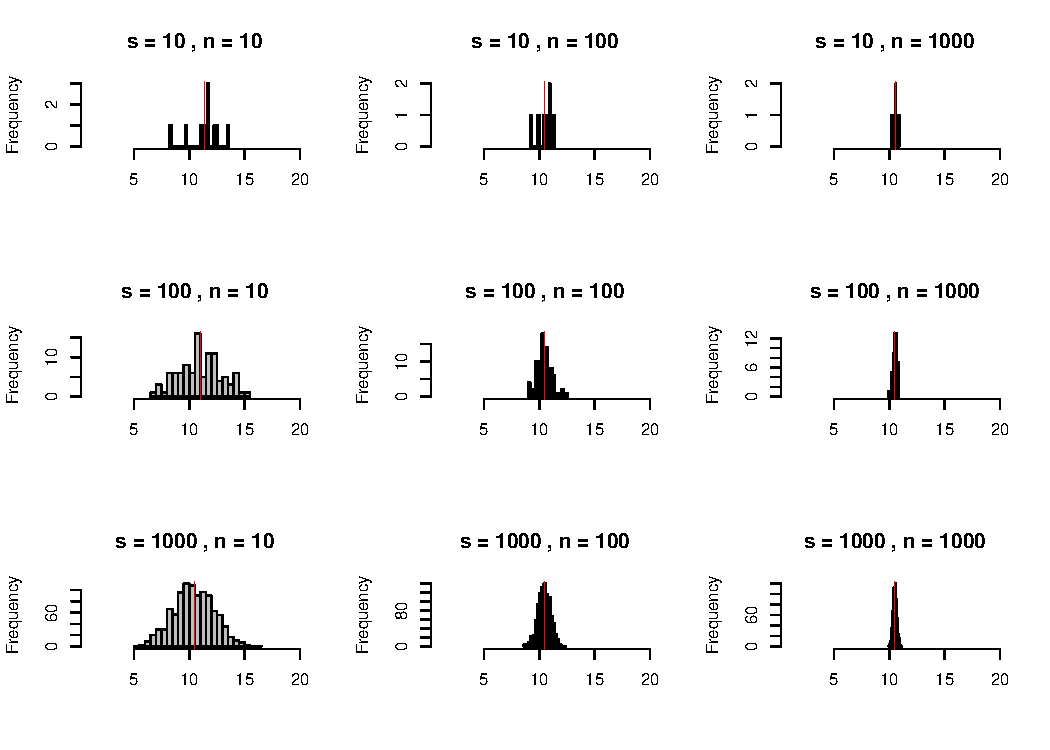
\includegraphics{problemset1_files/figure-pdf/unnamed-chunk-1-1.pdf}

\subsection{\texorpdfstring{\emph{Problem
b}}{Problem b}}\label{problem-b}

The histograms shows that when increasing the sample size reduces
variability in sample means. I set it to 1:20 so it's getting closer to
10. And increasing the number of samples makes it look like normal
distribution. The key assumption here is what CLT describes: the
distribution of a normalized version of the sample mean converges to a
standard normal distribution.

\section{2. Monte Carlo integration}\label{monte-carlo-integration}

\begin{Shaded}
\begin{Highlighting}[]
\NormalTok{func }\OtherTok{=} \ControlFlowTok{function}\NormalTok{(x)\{}\FunctionTok{exp}\NormalTok{(}\SpecialCharTok{{-}}\NormalTok{x)}\SpecialCharTok{*}\FunctionTok{sin}\NormalTok{(x)\}}
\NormalTok{result }\OtherTok{=} \FunctionTok{integrate}\NormalTok{(func, }\AttributeTok{lower =} \DecValTok{2}\NormalTok{, }\AttributeTok{upper =} \DecValTok{5}\NormalTok{)}
\FunctionTok{print}\NormalTok{(result)}
\end{Highlighting}
\end{Shaded}

\begin{verbatim}
0.03564528 with absolute error < 8.3e-16
\end{verbatim}

\section{3. Systematic and stochastic
components}\label{systematic-and-stochastic-components}

\subsection{\texorpdfstring{\emph{Problem
a}}{Problem a}}\label{problem-a-1}

Systematic Component: \(y_i=1+0.5x_{i1}-2.2x_{i2}+x_{i3}\) Stochastic
Component: \({\epsilon_i}\sim{N(\mu=0,\sigma^2=1.5)}\)

\subsection{\texorpdfstring{\emph{Problem
b}}{Problem b}}\label{problem-b-1}

\textbf{Part I.} The dimensions of \(\mathbf{X}\) is denoted as \(n\) is
\(2\).

\begin{Shaded}
\begin{Highlighting}[]
\NormalTok{data }\OtherTok{=} \FunctionTok{read.csv}\NormalTok{(}\StringTok{"xmat.csv"}\NormalTok{)}
\FunctionTok{print}\NormalTok{(}\FunctionTok{dim}\NormalTok{(data))}
\end{Highlighting}
\end{Shaded}

\begin{verbatim}
[1] 1000    3
\end{verbatim}

\begin{Shaded}
\begin{Highlighting}[]
\FunctionTok{head}\NormalTok{(data, }\DecValTok{10}\NormalTok{)}
\end{Highlighting}
\end{Shaded}

\begin{verbatim}
           X1 X2          X3
1  -4.8200977  1  1.54137265
2   2.5755430  0  1.25892647
3   0.3326820  1 -0.06933333
4  -1.1534374  1  0.07761559
5   2.0563184  0 -1.19921600
6   0.1335086  0  0.25054654
7   1.6025580  1 -0.41074599
8  -1.4491007  1  2.31999656
9   1.2676561  1 -0.80968744
10  1.0784026  1 -0.31089005
\end{verbatim}

\textbf{Part II.}

\begin{Shaded}
\begin{Highlighting}[]
\FunctionTok{set.seed}\NormalTok{(}\DecValTok{10825}\NormalTok{) }
\CommentTok{\# Why not 42 and 3407}
\NormalTok{coefficient\_0 }\OtherTok{=} \DecValTok{1}
\NormalTok{coefficient\_1 }\OtherTok{=} \FloatTok{0.5}
\NormalTok{coefficient\_2 }\OtherTok{=} \SpecialCharTok{{-}}\FloatTok{2.2}
\NormalTok{coefficient\_3 }\OtherTok{=} \DecValTok{1}
\NormalTok{x\_1 }\OtherTok{=}\NormalTok{ data}\SpecialCharTok{$}\NormalTok{X1}
\NormalTok{x\_2 }\OtherTok{=}\NormalTok{ data}\SpecialCharTok{$}\NormalTok{X2}
\NormalTok{x\_3 }\OtherTok{=}\NormalTok{ data}\SpecialCharTok{$}\NormalTok{X3}
\NormalTok{e }\OtherTok{=} \FunctionTok{rnorm}\NormalTok{(}\AttributeTok{n =} \FunctionTok{nrow}\NormalTok{(data), }\AttributeTok{mean =} \DecValTok{0}\NormalTok{, }\AttributeTok{sd =} \FunctionTok{sqrt}\NormalTok{(}\FloatTok{1.5}\NormalTok{))}
\NormalTok{y }\OtherTok{=}\NormalTok{ coefficient\_0 }\SpecialCharTok{+}\NormalTok{ coefficient\_1}\SpecialCharTok{*}\NormalTok{x\_1 }\SpecialCharTok{+}\NormalTok{ coefficient\_2}\SpecialCharTok{*}\NormalTok{x\_2 }\SpecialCharTok{+}\NormalTok{ coefficient\_3}\SpecialCharTok{*}\NormalTok{x\_3 }\SpecialCharTok{+}\NormalTok{ e}

\NormalTok{linear }\OtherTok{=} \FunctionTok{lm}\NormalTok{(y }\SpecialCharTok{\textasciitilde{}}\NormalTok{ x\_1 }\SpecialCharTok{+}\NormalTok{ x\_2 }\SpecialCharTok{+}\NormalTok{ x\_3)}
\FunctionTok{summary}\NormalTok{((linear))}
\end{Highlighting}
\end{Shaded}

\begin{verbatim}

Call:
lm(formula = y ~ x_1 + x_2 + x_3)

Residuals:
    Min      1Q  Median      3Q     Max 
-3.5330 -0.8196  0.0124  0.8168  4.5651 

Coefficients:
            Estimate Std. Error t value Pr(>|t|)    
(Intercept)  1.06651    0.05084   20.98   <2e-16 ***
x_1          0.48024    0.01925   24.95   <2e-16 ***
x_2         -2.26451    0.07852  -28.84   <2e-16 ***
x_3          0.95040    0.03822   24.86   <2e-16 ***
---
Signif. codes:  0 '***' 0.001 '**' 0.01 '*' 0.05 '.' 0.1 ' ' 1

Residual standard error: 1.225 on 996 degrees of freedom
Multiple R-squared:  0.6792,    Adjusted R-squared:  0.6782 
F-statistic: 702.9 on 3 and 996 DF,  p-value: < 2.2e-16
\end{verbatim}

\begin{Shaded}
\begin{Highlighting}[]
\CommentTok{\# Beautiful p{-}value}
\end{Highlighting}
\end{Shaded}

\section{4. OLS in matrix form}\label{ols-in-matrix-form}

\begin{Shaded}
\begin{Highlighting}[]
\FunctionTok{library}\NormalTok{(haven)}
\NormalTok{data\_2 }\OtherTok{=} \FunctionTok{read\_dta}\NormalTok{(}\StringTok{"coxappend.dta"}\NormalTok{)}
\FunctionTok{attributes}\NormalTok{(data\_2)}
\end{Highlighting}
\end{Shaded}

\begin{verbatim}
$class
[1] "tbl_df"     "tbl"        "data.frame"

$row.names
 [1]  1  2  3  4  5  6  7  8  9 10 11 12 13 14 15 16 17 18 19 20 21 22 23 24 25
[26] 26 27 28 29 30 31 32 33 34 35 36 37 38 39 40 41 42 43 44 45 46 47 48 49 50
[51] 51 52 53 54

$names
 [1] "var12"    "drop"     "year"     "enpv"     "enps"     "eneth"   
 [7] "ml"       "upper"    "enpres"   "proximit" "lnml"     "lmleneth"
[13] "smdp"     "smdpeth"  "multi"    "enpvlml"  "enpvUpp"  "multiV"  
[19] "enpvQ"    "enpvmult" "enpvsmdp" "proxpres" "drop2"   
\end{verbatim}

\begin{Shaded}
\begin{Highlighting}[]
\FunctionTok{head}\NormalTok{(data\_2, }\DecValTok{10}\NormalTok{)}
\end{Highlighting}
\end{Shaded}

\begin{verbatim}
# A tibble: 10 x 23
   var12      drop  year  enpv  enps eneth    ml upper enpres proximit  lnml
   <chr>     <dbl> <dbl> <dbl> <dbl> <dbl> <dbl> <dbl>  <dbl>    <dbl> <dbl>
 1 ARGENTINA     0  1985  3.37  2.37  1.34   9   0       2.51    0.550  2.20
 2 AUSTRALIA     0  1984  2.79  2.38  1.11   1   0       0       0      0   
 3 AUSTRIA       0  1986  2.72  2.63  1.01  30   0.115   2.27    0.800  3.40
 4 BAHAMAS       0  1987  2.11  1.96  1.34   1   0       0       0      0   
 5 BARBADOS      0  1986  1.93  1.25  1.50   1   0       0       0      0   
 6 BELGIUM       0  1985  8.13  7.01  2.35   8   0.401   0       0      2.08
 7 BELIZE        0  1984  2.06  1.60  3.46   1   0       0       0      0   
 8 BOLIVIA       1  1985  4.58  4.32  3.77  17.5 0       4.58    1      2.86
 9 BOTSWANA      0  1984  1.96  1.35  1.11   1   0       0       0      0   
10 BRAZIL        0  1990  9.68  8.69  2.22  30   0       5.69    0.630  3.40
# i 12 more variables: lmleneth <dbl>, smdp <dbl>, smdpeth <dbl>, multi <dbl>,
#   enpvlml <dbl>, enpvUpp <dbl>, multiV <dbl>, enpvQ <dbl>, enpvmult <dbl>,
#   enpvsmdp <dbl>, proxpres <dbl>, drop2 <dbl>
\end{verbatim}

\subsection{\texorpdfstring{\emph{Problem
a}}{Problem a}}\label{problem-a-2}

\begin{Shaded}
\begin{Highlighting}[]
\FunctionTok{print}\NormalTok{(}\FunctionTok{attributes}\NormalTok{(data\_2))}
\end{Highlighting}
\end{Shaded}

\begin{verbatim}
$class
[1] "tbl_df"     "tbl"        "data.frame"

$row.names
 [1]  1  2  3  4  5  6  7  8  9 10 11 12 13 14 15 16 17 18 19 20 21 22 23 24 25
[26] 26 27 28 29 30 31 32 33 34 35 36 37 38 39 40 41 42 43 44 45 46 47 48 49 50
[51] 51 52 53 54

$names
 [1] "var12"    "drop"     "year"     "enpv"     "enps"     "eneth"   
 [7] "ml"       "upper"    "enpres"   "proximit" "lnml"     "lmleneth"
[13] "smdp"     "smdpeth"  "multi"    "enpvlml"  "enpvUpp"  "multiV"  
[19] "enpvQ"    "enpvmult" "enpvsmdp" "proxpres" "drop2"   
\end{verbatim}

\begin{Shaded}
\begin{Highlighting}[]
\NormalTok{ols\_regression }\OtherTok{=} \ControlFlowTok{function}\NormalTok{(y, X) \{}
  \CommentTok{\# Add intercept to X}
\NormalTok{  X }\OtherTok{=} \FunctionTok{cbind}\NormalTok{(}\DecValTok{1}\NormalTok{, X)}
  
  \CommentTok{\# Calculate coefficients}
\NormalTok{  XtX }\OtherTok{=} \FunctionTok{t}\NormalTok{(X) }\SpecialCharTok{\%*\%}\NormalTok{ X}
\NormalTok{  XtX\_inv }\OtherTok{=} \FunctionTok{solve}\NormalTok{(XtX)}
\NormalTok{  XtY }\OtherTok{=} \FunctionTok{t}\NormalTok{(X) }\SpecialCharTok{\%*\%}\NormalTok{ y}
\NormalTok{  beta }\OtherTok{=}\NormalTok{ XtX\_inv }\SpecialCharTok{\%*\%}\NormalTok{ XtY}
  
  \CommentTok{\# Calculate residuals}
\NormalTok{  residuals }\OtherTok{=}\NormalTok{ y }\SpecialCharTok{{-}}\NormalTok{ X }\SpecialCharTok{\%*\%}\NormalTok{ beta}
  
  \CommentTok{\# Calculate variance}
\NormalTok{  n }\OtherTok{=} \FunctionTok{length}\NormalTok{(y)}
\NormalTok{  k }\OtherTok{=} \FunctionTok{ncol}\NormalTok{(X)}
\NormalTok{  sigma2 }\OtherTok{=} \FunctionTok{sum}\NormalTok{(residuals}\SpecialCharTok{\^{}}\DecValTok{2}\NormalTok{) }\SpecialCharTok{/}\NormalTok{ (n }\SpecialCharTok{{-}}\NormalTok{ k)}
  
  \CommentTok{\# Standard errors}
\NormalTok{  cov\_matrix }\OtherTok{=}\NormalTok{ sigma2 }\SpecialCharTok{*}\NormalTok{ XtX\_inv}
\NormalTok{  std\_errors }\OtherTok{=} \FunctionTok{sqrt}\NormalTok{(}\FunctionTok{diag}\NormalTok{(cov\_matrix))}
  
  \CommentTok{\# Create a results table}
\NormalTok{  results }\OtherTok{=} \FunctionTok{data.frame}\NormalTok{(}
    \AttributeTok{Coefficient =} \FunctionTok{as.vector}\NormalTok{(beta),}
    \AttributeTok{Std\_Error =}\NormalTok{ std\_errors}
\NormalTok{  )}
  \FunctionTok{rownames}\NormalTok{(results) }\OtherTok{=} \FunctionTok{c}\NormalTok{(}\StringTok{"Intercept"}\NormalTok{, }\FunctionTok{paste0}\NormalTok{(}\StringTok{"Var"}\NormalTok{, }\DecValTok{1}\SpecialCharTok{:}\NormalTok{(k }\SpecialCharTok{{-}} \DecValTok{1}\NormalTok{)))}
  
  \FunctionTok{return}\NormalTok{(results)}
\NormalTok{\}}
\end{Highlighting}
\end{Shaded}





\end{document}
